\documentclass[border=4pt]{standalone}
\usepackage{fontspec}
\setmainfont{TeX Gyre Heros}
\usepackage{tikz}
\usetikzlibrary{positioning,arrows.meta}
\definecolor{ink}{HTML}{1F1E1D}\definecolor{muted}{HTML}{6B6B6B}\definecolor{fill}{HTML}{EFEFEE}\definecolor{accent}{HTML}{3F6C8F}
\newcommand{\sub}{\fontsize{6.5bp}{8bp}\selectfont\color{muted}}
\begin{document}
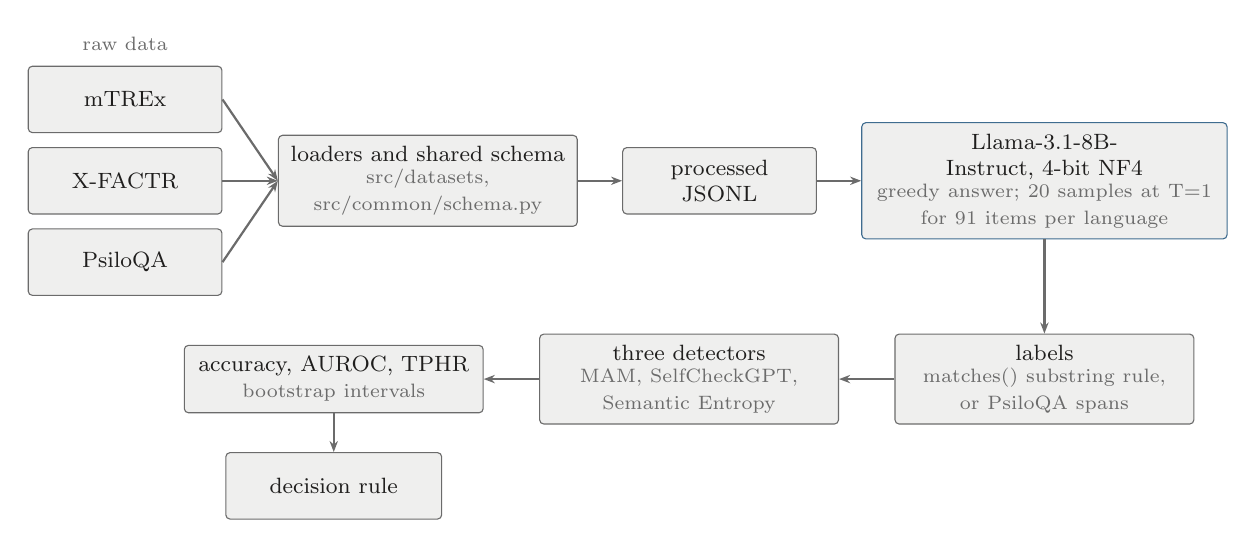
\begin{tikzpicture}[font=\fontsize{8bp}{9.5bp}\selectfont\color{ink},
 box/.style={draw=muted,fill=fill,rounded corners=1.5pt,align=center,inner sep=4pt,minimum height=24pt,text width=#1},
 box/.default=92pt, arr/.style={-{Stealth[length=4pt]},draw=muted,thick},
 note/.style={font=\fontsize{6.5bp}{8bp}\selectfont\color{muted},align=center}]
\node[box=62pt] (m) {mTREx};
\node[box=62pt,below=5pt of m] (x) {X-FACTR};
\node[box=62pt,below=5pt of x] (p) {PsiloQA};
\node[note,above=2pt of m] {raw data};
\node[box=100pt,right=20pt of x] (l) {loaders and shared schema\\{\sub src/datasets,\\src/common/schema.py}};
\node[box=62pt,right=16pt of l] (j) {processed JSONL};
\node[box=124pt,right=16pt of j,draw=accent] (g) {Llama-3.1-8B-Instruct, 4-bit NF4\\{\sub greedy answer; 20 samples at T=1\\for 91 items per language}};
\foreach \a in {m,x,p}{\draw[arr] (\a.east)--(l.west);}
\draw[arr](l)--(j);\draw[arr](j)--(g);
\node[box=100pt,below=34pt of g] (lab) {labels\\{\sub matches() substring rule,\\or PsiloQA spans}};
\node[box=100pt,left=20pt of lab] (det) {three detectors\\{\sub MAM, SelfCheckGPT,\\Semantic Entropy}};
\node[box=100pt,left=20pt of det] (met) {accuracy, AUROC, TPHR\\{\sub bootstrap intervals}};
\node[box=70pt,below=14pt of met] (dec) {decision rule};
\draw[arr](g.south)--(lab.north);
\draw[arr](lab)--(det);\draw[arr](det)--(met);\draw[arr](met)--(dec);
\end{tikzpicture}
\end{document}
